\begin{frame}{Motivation}
    \begin{figure}[h]
        \setcounter{subfigure}{0}
        \subfigure[Jeu vidéos]{
\includegraphics[height=.35\linewidth]{big_rigs}}
        \subfigure[Synthèse d’image]{
\includegraphics[height=.35\linewidth]{shrek4}}
        \subfigure[Éducation (\href{www.algodoo.com}{algodoo})]{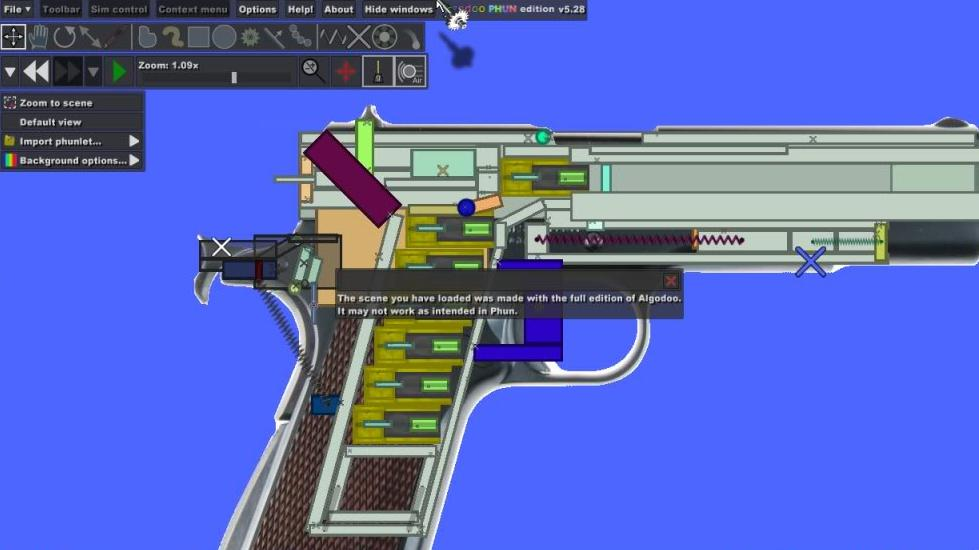
\includegraphics[height=.25\linewidth]{algodoo}}
    \end{figure}
\end{frame}

\begin{frame}{Moteurs open-source célèbres (ou pas)}
    \begin{itemize}
        \item \textbf{2D:} Box 2d (Erin Catto)
            \begin{center}
                
\includegraphics[height=.15\linewidth]{box2d}
            \end{center}
        \item \textbf{3D:} Bullet physics (Erwin Courmand)
            \href{http://www.bulletphysics.org/Bullet/phpBB3/}{www.bulletphysics.org}
            \begin{center}
                
\includegraphics[height=.15\linewidth]{bullet_physics}
            \end{center}
            \pause
        \item \textbf{2D et 3D (générique):} Pas du tout célèbre, mais existe!
    \end{itemize}
\end{frame}

\begin{frame}{Les objets rigides}
    \begin{itemize}
        \item Objects non déformables.
        \item Peut être assimilé à un point pour les translations.
    \end{itemize}
    \begin{figure}[h]
        \setcounter{subfigure}{0}
        \subfigure[Objet rigide]{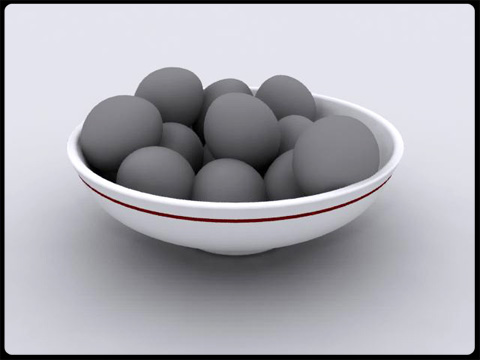
\includegraphics[height=.35\linewidth]{rigid_body}}
        \subfigure[Objet déformable]{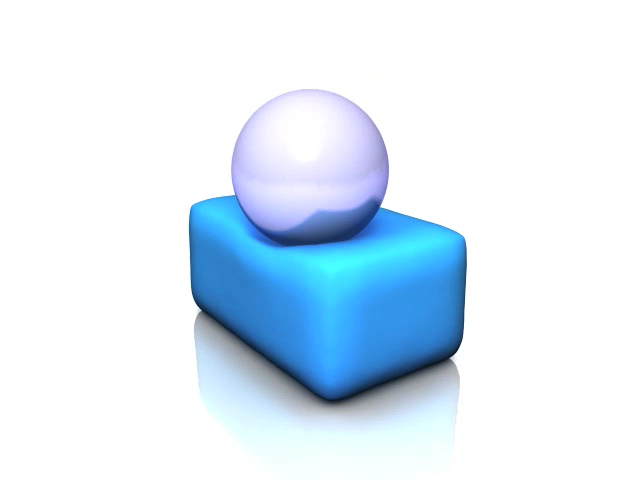
\includegraphics[height=.35\linewidth]{deformable}}
    \end{figure}
\end{frame}

\begin{frame}{Ce qui ne sera pas abordé}
    \begin{figure}[h]
        \setcounter{subfigure}{0}
        \subfigure[Joints]{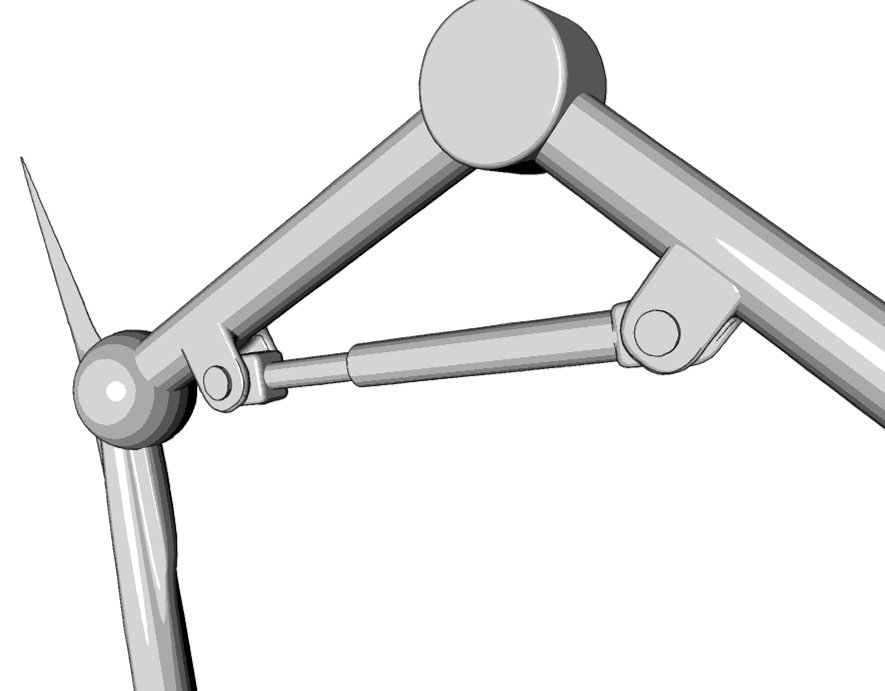
\includegraphics[height=.25\linewidth]{joint}}
        \pause
        \subfigure[Soft bodies]{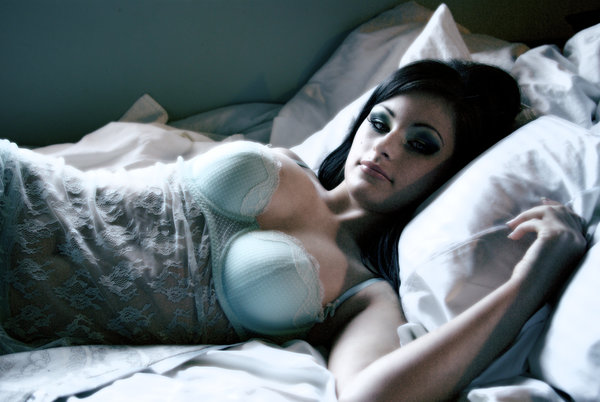
\includegraphics[height=.25\linewidth]{soft_body}}
        \pause
        \subfigure[Lancer de rayons]{
\includegraphics[height=.25\linewidth]{ray_casting}}
    \end{figure}
\end{frame}
